% Copyright (c)  2005-2010 EDF-EADS-PHIMECA.
% Permission is granted to copy, distribute and/or modify this document
% under the terms of the GNU Free Documentation License, Version 1.2
% or any later version published by the Free Software Foundation;
% with no Invariant Sections, no Front-Cover Texts, and no Back-Cover
% Texts.  A copy of the license is included in the section entitled "GNU
% Free Documentation License".
\renewcommand{\filename}{docUC_InputWithData_KernelSmoothing.tex}
\renewcommand{\filetitle}{UC : PDF fitting by kernel smoothing and graphical validation : superposition of the empirical and kernel smoothing CDF}

% \HeaderNNIILevel
% \HeaderIILevel
\HeaderIIILevel


\index{Distribution!Kernel mixture}
\index{Fitting Distribution!Kernel smoothing}
\index{Graph!Empirical cumulative density function}
\index{Graph!PDF-CDF curves}
\index{Graph Manipulation!Bounding box}
\index{Graph Manipulation!ViewImage}
\index{Graph Manipulation!Show}
\index{Graph!Superposition empirical - kernel smoothed CDF}

The objective of this Use Case is to model the PDF of a random  vector, described by a numerical sample thanks to the kernel smoothing method and to superpose on the same graph the kernel smoothing PDF and the histogram built from the same numerical sample.\\



Details on the kernel smoothing method may be found in the Reference Guide (\href{OpenTURNS_ReferenceGuide.pdf}{see file Reference Guide - Step B -- Kernel Smoothing}).\\

Details on each object may be found in the User Manual  (\href{OpenTURNS_UserManual_TUI.pdf}{see User Manual - Probabilistic modeling / Linear combination of probability density functions}).\\

In dimension 1, the kernel smoothed probability density function $\hat{p}$ has the following expression, where $K$ is the univariate kernel, $n$ the numerical sample size and $(X_1, \cdots, X_n) \in \mathbb{R}^n$ the univariate random sample with $\forall i, \, \, X_i \in \mathbb{R}$ :
\begin{equation}
  \label{kernelSmooth}
  \hat{p}(x) = \displaystyle \frac{1}{nh}\sum_{i=1}^{n} K\left(\frac{x-X_i}{h}\right)
\end{equation}
The kernel $K$ is a function satisfying $\int K(x)\, dx=1$. Usually, $K$ is chosen to be a unimodal probability density fucntion that is symmetric about 0.\\
The parameter $h$ is called the \emph{bandwidth}.\\


In dimension 1, the boundary effects may be taken into account in Open TURNS : the boundaries are automatically detected from the numerical sample (with the $min$ and $max$ functions) and the kernel smoothed PDF is corrected in the boundary areas to remain within the boundaries, according to the miroring technique :
\begin{itemize}
\item the Scott bandwidth is evaluated from the numerical sample : $h$
\item two subsamples are extracted from the inital numerical sample, containing all the points within the range $[min, min + h[$ and  $]max-h, max]$,
\item both subsamples are transformed into their symmetric samples with respect their respective boundary : its results two samples within the range  $]min-h, min]$ and  $[max, max+h[$,
\item a kernel smoothed PDF is built from the new numerical sample composed with the initial one and the two new ones, with the previous bandwidth $h$,
\item this last kernel smoothed PDF is truncated within the inital range  $[min, max]$ (conditionnal PDF).
\end{itemize}
The choice of the kind of the kernel is free in Open TURNS : it is possible to select any 1D distribution and to define it as a kernel. However, in order to optimize the efficiency of the kernel smoothing fitting (it means to minimise the AMISE error), it is recommended to select a {\bf symmetric distribution} for the kernel. \\
All the distribution default constructors of Open TURNS create a symmetric default distribution when possible. It is also possible to work with the Epanechnikov kernel, which is a $Beta(r=2, t=4, a=-1, b=1)$. \\
The default kernel is a product of standard Normal distribution. The dimension of the product is automatically evaluated from the random sample.\\

The bandwidth $\vect{h}$ may be fixed by the User. However, it is recommended to let Open TURNS evaluate it automatically from the numerical sample according to the following rules :
\begin{itemize}
\item In dimension $d$, Open TURNS automatically applies the Scott rule.
\item In dimension 1, the automatic bandwidth selection method depends  on the size $n$ of the numerical sample. As a matter of fact, the computation bottleneck is the estimation of the estimators $\hat{\Phi}_r$ as it requires the evaluation of a double summation on the numerical sample, which has a cost of $\mathcal{O}(n^2)$.
  \begin{itemize}
  \item if $n \leq 250$, the Solve-the-equation  plug-in method is used on the entire numerical sample.
  \item if $n>250$, the Solve-the-equation  plug-in method is too computationnally expensive. Then, Open TURNS proceeds as follows :the plug-in method on the entire numerical sample if its size is inferior to 250; the mixted method in the other case. Refer to the Reference Guide in order to have details on these methods (see refernec Guide to have detials on methods).
  \end{itemize}
\end{itemize}


It is possible to specify a particular bandwidth, evaluated according to one of the previous rules as follows :
\begin{itemize}
\item \emph{computeSilvermanBandwidth} applies the Silverman rule,
\item \emph{computePluginBandwidth} applies the plug-in method on the entire numerical sample,
\item \emph{computeMixedBandwidth} applies the mixted plug-in method on the entire numerical sample, as described above.
\end{itemize}

\textspace\\
\requirements{
  \begin{description}
  \item[$\bullet$] a nD-sample : {\itshape sample}
  \item[type:]  NumericalSample
  \end{description}
}
{
  \begin{description}
  \item[$\bullet$] a kernel smoothed distribution : {\itshape kernelSmoothedDist}
  \item[type:]  Distribution
  \end{description}
}

\textspace\\
Python script for this UseCase :

\begin{lstlisting}
  ##################################
  # STEP 1 : Creation of the kernel

  # Create the default kernel : kernel product of N(0.0, 1.0)
  kernel = KernelSmoothing()

  # Create a specified kernel
  # for example, a Uniform one
  # the default construction of the Uniform
  # creates the Uniform(-1.0, 1.0)
  kernel = KernelSmoothing(Uniform())

  # Specify totally the kernel
  # CARE : the kernel smoothing is more efficient
  # when the kernel support is symmetric qith respect to 0
  myDist = Triangular(-2.0, 0.0, 2.0)
  kernel = KernelSmoothing(myDist)


  #####################################################
  # STEP 2 : Creation of the kernel smoothed distribution
  # The dimension of the distribution is authomatically
  # detected from the numerical sample

  # Metod 1 : With no bandwidth specification : the method employed is
  # adapted to the size of the numerical sample
  # With no boudary treatment
  kernelSmoothedDist = kernel.build(sample)

  # Check the bandwidth used
  print  "kernel bandwidth=" , kernel.getBandwidth()

  # Method 2 : Specify a particular bandwidth evaluated
  #  according to the Silverman rule
  myBandwith = kernel.computeSilvermanBandwidth(sample)

  # or according to the plug-in method
  # applied in the entire numerical sample
  myBandwith = kernel.computePluginBandwidth(sample)

  # or according to the mixted plug-in method
  myBandwith = kernel.computeMixedBandwidth(sample)

  # Then build the estimation with the specified bandwidth
  kernelSmoothedDist = kernel.build(sample, myBandwith)

  # Add a boundary treatment
  # CARE : only in dimension 1
  kernelSmoothedDist = kernel.build(sample, True)
  # or
  kernelSmoothedDist = kernel.build(sample, myBandwith, True)


  # GRAPH : In dimension 1, superposition of the kernel smoothed CDF
  # and the empirical CDF
  # Create the graph containing the  kernel smoothed PDF
  kernelSmoothedCDF = kernelSmoothedDist.drawCDF()

  # Draw the empirical CDF of the sample on the same graph
  empiricalCDF = VisualTest.DrawEmpiricalCDF(sample,sample.getMin()[0],sample.getMax()[0])
  drawableEmpiricalCDF = empiricalCDF.getDrawable(0)

  # Add the second drawable on the first graph
  kernelSmoothedCDF.add(drawableEmpiricalCDF)

  # Impose a bounding box : x-range and y-range
  # boundingBox = [xmin, xmax, ymin, ymax]
  myBoundingBox = NumericalPoint( (xmin, xmax, ymin, ymax) )
  kernelSmoothedCDF.setBoundingBox(myBoundingBox)

  # In order to see the graph without creating the associated files
  Show(kernelSmoothedCDF)

  # Draw the final graph on the file smoothedCDF-EmpiricalCDF at format .eps, .png and .fig
  # if the adress is not fulfilled, the file is created in the current directory
  kernelSmoothedCDF.draw("smoothedCDF-EmpiricalCDF")

  # View the bitmap file
  ViewImage(kernelSmoothedCDF.getBitmap())

  # Check the adress of the bitmap and Postscript files
  print "bitmap=", kernelSmoothedCDF.getBitmap()
  print"postscript=", kernelSmoothedCDF.getPostscript()
\end{lstlisting}
\textspace\\


Figures \ref{pdf_KernelSmooth} and \ref{cdf_KernelSmooth}  show a 1D kernel smoothing of a distribution of type Mixture which PDF is defined by : 0.2*Triangular(1.0, 2.0, 4.0) + 0.5*Normal(-1.0, 1.0) + 0.3*Exponential(1.0, 3.0), thanks to a numerical sample of size $10^4$, with a Normal,  Triangular and Epanechnikov kernel, when the  bandwidth is selected according to the mixted plug-in method.\\

Figures \ref{pdf_KernelSmoothBWSel} and \ref{cdf_KernelSmoothBWSel} show the difference when the previous distribution is estimated with  a Normal kernel and when the bandwidth is selected according to the Silverman rule, the plug-in method or the mixted plug-in method, thanks to a numerical sample of size $10^3$.\\

Figures \ref{pdf_KernelSmooth_boundary} and \ref{cdf_KernelSmooth_boundary} show the effect of the boundary treatment in the kernel smoothing through the example of the exponential distribution $Exp(\lambda = 2.0, \gamma = 0.0)$. A Normal kernel is used and the  bandwidth is selected according to the mixted plug-in method, thanks to a numerical sample of size $10^4$.


\begin{figure}[H]
  \begin{minipage}{7cm}
    \begin{center}
      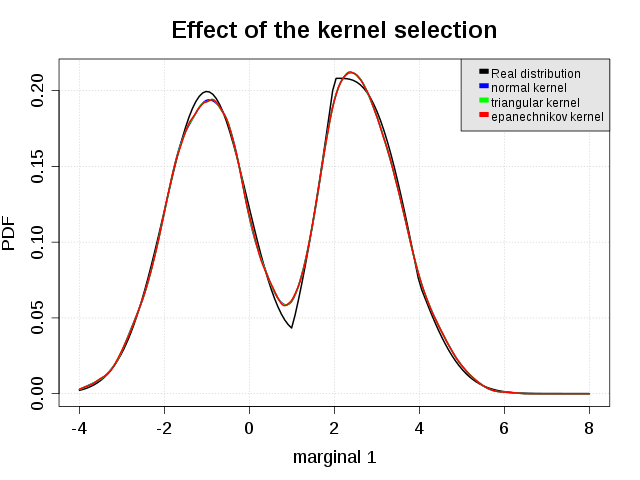
\includegraphics[width=7cm]{kernelSmoothing_pdf.png}
      \caption{PDF of th kernel smoothed distribution and of the real one with different kernels.}
      \label{pdf_KernelSmooth}
    \end{center}
  \end{minipage}
  \hfill
  \begin{minipage}{7cm}
    \begin{center}
      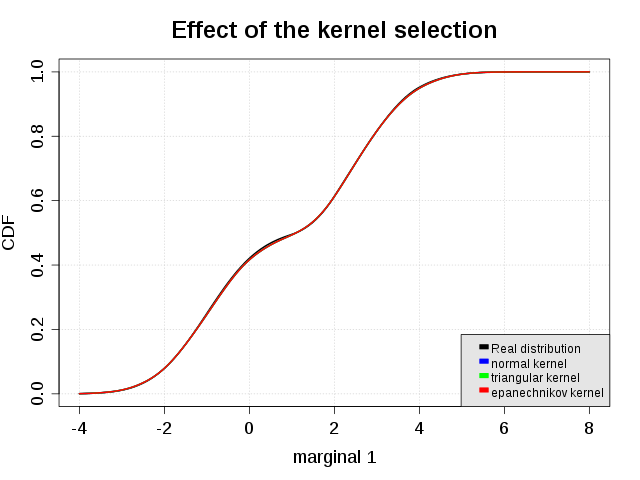
\includegraphics[width=7cm]{kernelSmoothing_cdf.png}
      \caption{CDF of the kernel smoothed distribution and of the real one with different kernels.}
      \label{cdf_KernelSmooth}
    \end{center}
  \end{minipage}
\end{figure}


\begin{figure}[H]
  \begin{minipage}{7cm}
    \begin{center}
      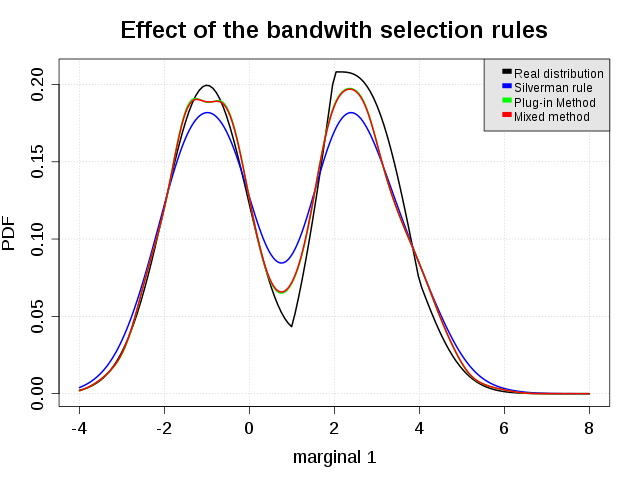
\includegraphics[width=7cm]{kernelSmoothingBWSel_pdf.png}
      \caption{PDF of the kernel smoothed distribution and of the real one with different bandwidth selection rules.}
      \label{pdf_KernelSmoothBWSel}
    \end{center}
  \end{minipage}
  \hfill
  \begin{minipage}{7cm}
    \begin{center}
      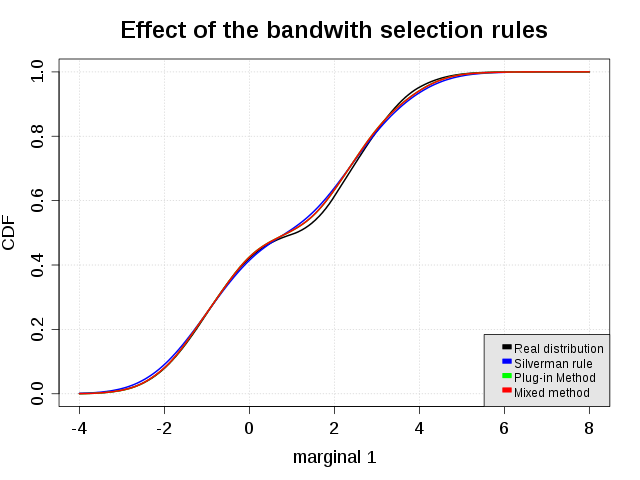
\includegraphics[width=7cm]{kernelSmoothingBWSel_cdf.png}
      \caption{CDF of the kernel smoothing distributions and of the real one with different bandwidth selection rules.}
      \label{cdf_KernelSmoothBWSel}
    \end{center}
  \end{minipage}
\end{figure}

\begin{figure}[H]
  \begin{minipage}{7cm}
    \begin{center}
      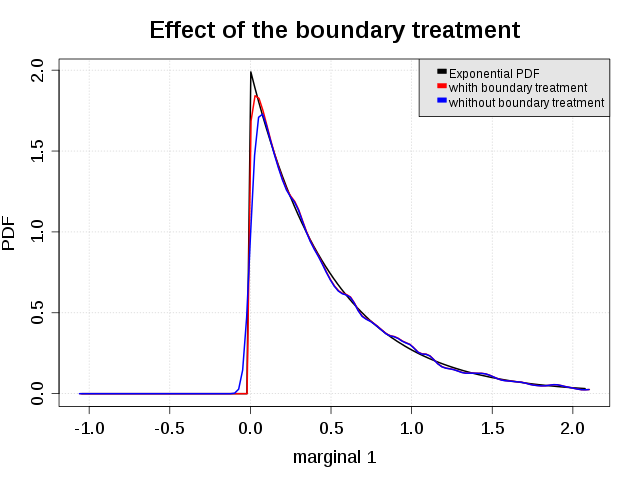
\includegraphics[width=7cm]{kernelSmoothing_boundary_pdf.png}
      \caption{Effect of the boundary treatment on the kernel smoothing PDF of an exponential distribution.}
      \label{pdf_KernelSmooth_boundary}
    \end{center}
  \end{minipage}
  \hfill
  \begin{minipage}{7cm}
    \begin{center}
      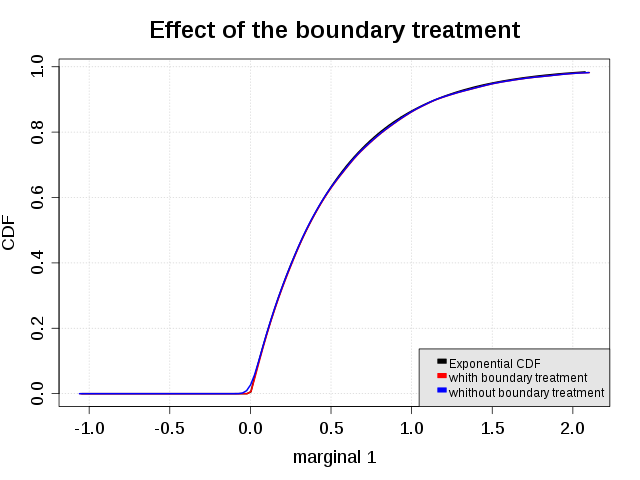
\includegraphics[width=7cm]{kernelSmoothing_boundary_cdf.png}
      \caption{Effect of the boundary treatment on the kernel smoothing CDF of an exponential distribution.}
      \label{cdf_KernelSmooth_boundary}
    \end{center}
  \end{minipage}
\end{figure}
